% -*- TeX -*- -*- UK -*- -*- BMR -*-
% ----------------------------------------------------------------
% Beamer presentation ************************************************
%
% Subhaneil Lahiri's template
%
% To compile:
%   Ctrl-Shift-P
%
% **** -----------------------------------------------------------
\documentclass{beamer}%[hyperref={backref=slide}]

\input{sl_slide_preamble.tex}
\input{sl_slide_graphics_preamble.tex}
\input{sl_definitions.tex}
\input{sl_slide_symbols.tex}
\graphicspath{{"Figures/"}}
\DeclareMathOperator{\SNR}{SNR}
\DeclareMathOperator{\snr}{SNR}
%matrices
\newcommand{\I}{\mathbf{I}}
%prob vector
\newcommand{\pr}{\mathbf{p}}
%equilibrium distribution
\newcommand{\eq}{\pr^\infty}
%other symbols
\newcommand{\w}{\mathbf{w}}
\newcommand{\W}{\mathbf{W}}
\newcommand{\frg}{\W^\mathrm{F}}
\newcommand{\M}{\mathbf{M}}
\newcommand{\F}{\boldsymbol{\Phi}}
\newcommand{\wv}{\vec{w}}
%super/subscripts
\newcommand{\pot}{^{\text{pot}}}
\newcommand{\dep}{^{\text{dep}}}
\newcommand{\potdep}{^{\text{pot/dep}}}
\newcommand{\lmax}{_{\text{max}}}
\newcommand{\lmin}{_{\text{min}}}
%quantities
\newcommand{\initial}{\mathcal{I}}
\newcommand{\area}{\mathcal{A}}
\renewcommand{\e}{\mathsf{e}}
%---------Title-----------------------------------------------------------

\title[Complex synapses]{A general theory of learning and memory with Complex Synapses}
%
\subtitle{\small{based on work with Surya Ganguli}
}
%
\author{Subhaneil Lahiri%\inst{1}
}
%
\institute[Stanford]{%
%\inst{1}
Stanford University, Applied Physics
}
%
%\slideCaption{}

%---------Beginning--------------------------------------------------------

\begin{document}

%-------------Slide--------------------------------------------------------

\begin{frame}
%
 \titlepage
%
\end{frame}

%-------------Slide--------------------------------------------------------

\begin{frame}{Introduction}
%
 We often model synaptic plasticity as the change of a single number (synaptic weight).
 \note[item]{amplitude of psp.}
 In reality, there is a complex dynamical system inside a synapse.

 \vp Semi-realistic models of synaptic memory have terrible storage without synaptic complexity.
 \note[item]{finite number of values.}

 \vp We will study the entire space of a broad class of models of complex synapses to find upper bounds on their performance.

%
\end{frame}

%-------------Slide--------------------------------------------------------

\begin{frame}{Outline}
%
 \tableofcontents[hideallsubsections]
 \note[item]{review terrible properties of simple synapses.}
 \note[item]{mathematical formalism of model, quantify performance (memory decay over time)}
 \note[item]{upper bounds on single numbers that describe performance at all times}
 \note[item]{upper bounds at finite times}
%
\end{frame}

%-------------Section--------------------------------------------------------

\section{Why complex synapses?}

%-------------Slide--------------------------------------------------------

\begin{frame}[label=fr_net]{Complex synapse}
%
 \begin{center}
 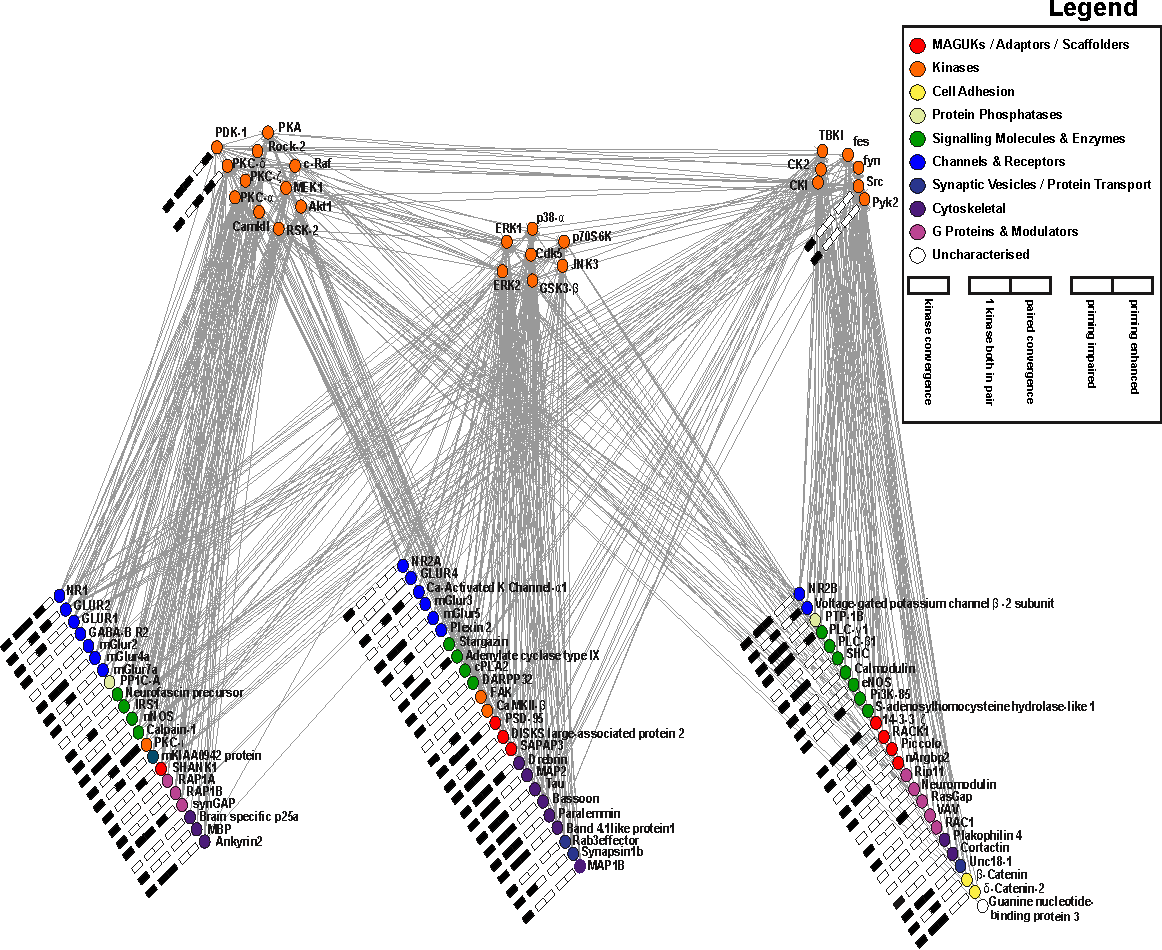
\includegraphics[height=6cm]{2000102CobaFig4.pdf}\citerrr{Coba2009phosphorylation}
 \end{center}
 \hyperlink{fr_questions}{There} is a complex, dynamical molecular network underlying synaptic plasticity.
 \note[item]{Does this matter?}
 \note[item]{Could just be the machinery for changing synaptic weight}
 \note[item]{link back to questions on ``There''}
%
\end{frame}

%-------------Slide--------------------------------------------------------

\begin{frame}{Storage capacity of synaptic memory}
%
  A classical perceptron (used as a recognition memory device) has a capacity $\propto N$, the number of synapses.

 \vp Requires synapses' dynamic range also $\propto N$.

 \vp If we restrict synaptic weight to a fixed, finite set of values,\\
 \hp $\implies$ tradeoff between learning and forgetting:\\
 \hp new memories overwriting old.

 \vp If we wish to store new memories rapidly, memory capacity  $\sim\CO(\log N)$.
 \\ \citerr{amit1992constraints,amit1994learning}

 \vp To circumvent this tradeoff, need to go beyond model of a synapse as a single number.
%
\end{frame}

%-------------Section--------------------------------------------------------

\section{Modelling synaptic complexity}

%-------------Slide--------------------------------------------------------

\begin{frame}{Complex synapses}
%
  \aligntop{\includegraphics[width=5cm]{synapse.svg}}
  \hp\aligntop{\includegraphics[width=2cm]{pot.svg}}
  \hp\aligntop{\includegraphics[width=2cm]{dep.svg}}
%
\end{frame}

%-------------Slide--------------------------------------------------------

\begin{frame}{Simplifying assumptions}
%
\begin{itemize}
  \item There are $N$ identical synapses with $M$ internal functional states.
  \item States of different synapses are independent of each other.
  \item Which synapses eligible for plasticity chosen randomly.
  \item Potentiating/depressing plasticity events $\sim$ Poisson processes with rates $rf\potdep$, where $f\pot+f\dep=1$.
      \note{In other words, $r$ is the total rate of plasticity events per synapse and $f\potdep$ are the fraction of these events that are potentiating/depressing.}
  \item Potentiation and depression are described by Markov processes with transition probabilities $\M\potdep$.
  \item Synaptic weights of the internal states are given by vector $\w$.\\ Can only take values $\pm1$.
\end{itemize}
%
\end{frame}

%-------------Slide--------------------------------------------------------

\begin{frame}{Probabilities}
%
 At $t=0$, the memory is created by $\M\potdep$ with probability $f\potdep$.
 \note[item]{for this one, we keep track of pot/dep}

 \vp Forgetting caused by subsequent memories, evolving as
 %
 \begin{equation*}
   \diff{\pr(t)}{t} = r\pr(t)\frg,
   \qquad
   \frg = f\pot\M\pot+f\dep\M\dep-\I,
 \end{equation*}
 %
 \note[item]{$\frg$ is forgetting matrix, don't keep track of pot/dep}
 Eventually, this will settle into the equilibrium distribution:
 %
 \begin{equation*}
   \eq\frg=0.
 \end{equation*}
 %
 \note[item]{In equilibrium prior to memory creation}
%
\end{frame}

%-------------Slide--------------------------------------------------------

\begin{frame}{Memory curve}
%
 $\wv$ is the $N$-element vector of synaptic weights.
 \note[item]{of different synapses}
  %
 \begin{equation*}
   \begin{aligned}
     \text{Signal} &= \av{\wv_\text{ideal} \cdot \wv(t) -  \wv_\text{ideal} \cdot \wv(\infty)}\\
     \text{Noise} &= \var\prn{\wv_\text{ideal} \cdot \wv(\infty)}
   \end{aligned}
 \end{equation*}
 %
 \note[item]{ideal: pot$\to$strong...}
 \note[item]{if we ignore correlations...}
 Related to reconstruction probability of single synapses.
 %
 \begin{equation*}
   \SNR(t) \sim \sqrt{N}\,P(\text{strong/weak},t|\text{pot/dep},t=0)-\ldots(t=\infty).
 \end{equation*}
 %

%
\end{frame}

%-------------Slide--------------------------------------------------------

\begin{frame}{Example models}
%
 Two example models of complex synapses.
 \begin{center}
% \parbox[t]{30cm}{
  \aligntop{\includegraphics[width=4cm]{cascade.svg}}
  \hspace{2cm}
  \aligntop{\includegraphics[width=4cm]{multistate.svg}}
% }
 \end{center}
 \citerr{Fusi2005cascade,amit1994learning,Fusi2007multistate}

 These have different memory storage properties
 \begin{center}
 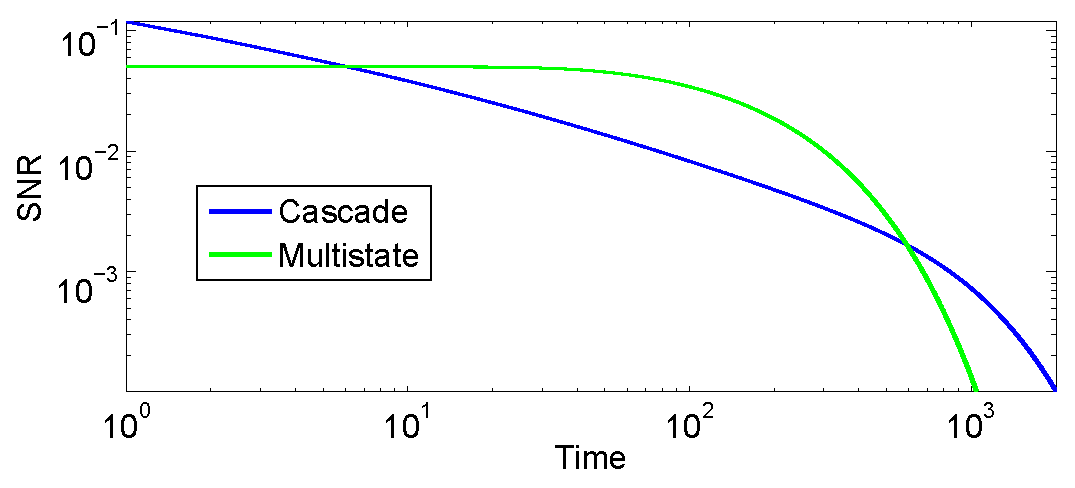
\includegraphics[width=8cm]{cascms.eps}
 \end{center}
%
\end{frame}

%-------------Slide--------------------------------------------------------

\begin{frame}[label=fr_questions]{Questions}
%
 \begin{itemize}
   \item Can we understand the space of \emph{all possible} synaptic models?
   \note[item]{not just individual models}
   \item How does structure \hyperlink{fr_net<1>}{(topology)} of model $\to$ function (memory curve)?
   \note[item]{understand net (link on topology)}
   \item What are the limits on what can be achieved?
   \note[item]{avoid using word ``optimal''. depends on what want to do.}
   \item Which transition topologies saturate these limits?
 \end{itemize}
%
\end{frame}

%-------------Slide--------------------------------------------------------

\begin{frame}{Memory curve 2}
%
 Memory curve given by
 %
 \begin{equation*}
   \snr(t) = \frac{\sqrt{N}(2f\pot f\dep)}{\sqrt{\eq_+\eq_-}}\, \eq \prn{\M\pot-\M\dep}
      \exp\prn{rt\frg}\w.
 \end{equation*}
 %
 \note[item]{prefactors don't do anything, ignore}
 \note[item]{prior state, encoding, forgetting, readout}
 Constraints: \qquad $\M\potdep_{ij}\in[0,1]$, \qquad $\sum_j\M\potdep_{ij}=1$.
 \note[item]{difficult to to apply}
 
 \vp Eigenmode decomposition:
 %
 \begin{equation*}
   \snr(t) = \sqrt{N}\sum_a \initial_a \,\e^{-rt/\tau_a}.
 \end{equation*}
 %
 \note[item]{what are constraints on these?}
%
\end{frame}


%-------------Section--------------------------------------------------------

\section{Upper bounds}

%-------------Section--------------------------------------------------------

\subsection{Initial SNR}


%-------------Slide--------------------------------------------------------

\begin{frame}{Initial SNR as flux}
%
 Initial SNR is closely related to flux between strong \& weak states
 %
 \begin{equation*}
   \SNR(0) \leq \frac{4\sqrt{N}}{r}\,\F_{-+}.
 \end{equation*}
 %
 \note[item]{usually saturated: pot never dec, dep never inc}
 Max when {\parbox[t]{8cm}{potentiation guarantees $\w\to+1$,\\ 
 depression guarantees $\w\to-1$.}}
%
\end{frame}


%-------------Slide--------------------------------------------------------


%-------------Section--------------------------------------------------------

\section{Envelope memory curve}

%-------------Slide--------------------------------------------------------






%-------------Slide--------------------------------------------------------
%
%% Press Ctrl-D to insert a new slide
%
%
%-------------Slide--------------------------------------------------------

\begin{frame}{Acknowledgements}
%
 Thanks to:
 \begin{itemize}
   \item Surya Ganguli
   \item Stefano Fusi
   \item Marcus Benna
 \end{itemize}
 \note[item]{Last slide!}
%
\end{frame}

%-------------Slide--------------------------------------------------------

\begin{frame}[allowframebreaks]{References}
%

 {\small
 \bibliographystyle{unsrt_slides}
 \bibliography{maths,neuro}
 }
%
\end{frame}


%-----End----------------------------------------------------------------

\end{document}
